\documentclass[12pt]{article}

% Packages
\usepackage[margin=1in]{geometry}
\usepackage{fancyhdr}
\usepackage{hyperref}
\usepackage{datetime} % For formatting the current date
\usepackage{parskip} % Adds space between paragraphs and removes paragraph indents
\usepackage{amsmath}
\usepackage{amssymb}
\usepackage{graphicx}


% Hyperlink settings
\hypersetup{
    colorlinks=true, % Colored links instead of boxes
    urlcolor=blue,   % Blue color for external links
}

% Custom date format
\newdateformat{monthyeardate}{%
\monthname[\THEMONTH] \THEYEAR}

% Header settings
\pagestyle{fancy}
\fancyhf{} % Clear all header and footer fields
\lhead{MATH 440 \\ 2:00 PM - 3:20 PM} % Left header with class number and time
\rhead{Marty Martin \\ \monthyeardate\today} % Right header with your name and the date
\renewcommand{\headrulewidth}{0.4pt} % Header underlining
\setlength{\headheight}{54pt} % Ensure there's enough space for two lines in the header

\begin{document}

\begin{center}
  \Large \textbf{Homework 12}
\end{center}

\section*{Problem 4.3.10}
\subsection*{Question}
The basketball team at State Tech, named the Fighting Logarithms, has a 70\%  foul-shooting percentage.
\begin{itemize}
    \item (a) Write a formula for the exact probability that out of their next one hundred free throws, they will make between seventy-five and eighty, inclusive.
    \item (b) Approximate the probability asked for in part (a).
\end{itemize}

\subsection*{Solution}
\subsubsection*{Part (a): Exact Probability}
% Considering a binomial distribution where each free throw is an independent trial
% n = number of trials, p = probability of success on each trial
\[
P(X = k) = \binom{n}{k} p^k (1-p)^{n-k}
\]
\[
P(75 \leq X \leq 80) = \sum_{k=75}^{80} \binom{100}{k} (0.7)^k (0.3)^{100-k}
\]
% This calculates the probability of exactly k successes in n trials, summed from 75 to 80

\subsubsection*{Part (b): Approximation using the Normal Distribution and Z-table}
% Calculate the Z-scores for the lower and upper bounds
\[
Z_{lower} = \frac{75 - 70}{4.5826} \approx 1.091
\]
\[
Z_{upper} = \frac{80 - 70}{4.5826} \approx 2.182
\]
% Using the Z-table to find probabilities for Z_{lower} and Z_{upper}

For Z = 1.09, the table gives a probability of 0.8621

For Z = 2.18, the table gives a probability of 0.9854
% The probability P(75 \leq X \leq 80) is then
\[
P(75 \leq X \leq 80) \approx 0.9854 - 0.8621 = 0.1233
\]
% This value is obtained by subtracting the cumulative probability of Z_{lower} from Z_{upper}

\newpage

\section*{Problem 4.3.18}
\subsection*{Question}
Suppose \(X_1, X_2, X_3,\) and \(X_4\) are independent Poisson random variables, each with parameter \(\lambda = 3\). Define \(S = X_1 + X_2 + X_3 + X_4\).
\begin{itemize}
    \item (a) Use the properties of Poisson processes to find the distribution of \(S\).
    \item (b) Calculate the probability \(P(13 \leq S \leq 14)\) exactly and approximate it using the Central Limit Theorem.
\end{itemize}

\subsection*{Solution}
\subsubsection*{Part (a): Finding the Distribution of \(S\)}
% Since S is the sum of four independent Poisson random variables each with parameter 3,
% the sum will also be a Poisson random variable whose parameter is the sum of the individual parameters.
\[
\lambda_S = 3 + 3 + 3 + 3 = 12
\]
% Therefore, S ~ Poisson(12).

\subsubsection*{Part (b): Approximation using the Central Limit Theorem}
% Standardizing the scores for S = 13 and S = 14
\[
Z_{13} = \frac{13 - 12}{\sqrt{12}} \approx 0.2887
\]
\[
Z_{14} = \frac{14 - 12}{\sqrt{12}} \approx 0.5774
\]
% Using the Z-table to find the cumulative probabilities for these Z-scores
% Assuming the closest values from the Z-table are:
\[
P(Z \leq 0.29) \approx 0.6141 \quad \text{(for } Z_{13}\text{)}
\]
\[
P(Z \leq 0.58) \approx 0.7186 \quad \text{(for } Z_{14}\text{)}
\]
% Calculating the probability that S is between 13 and 14 using the approximated values from the Z-table
\[
P(13 \leq S \leq 14) \approx P(Z \leq 0.5774) - P(Z \leq 0.2887) = 0.7186 - 0.6141 = 0.1045
\]
% This value represents the probability that S, the sum of four independent Poisson random variables,
% falls between 13 and 14, using the normal approximation.


\newpage

\section*{Problem 4.3.26}
\subsection*{Question}
The cross-sectional area of plastic tubing for use in pulmonary resuscitators is normally distributed with mean \( \mu = 12.5 \) mm\(^2\) and standard deviation \( \sigma = 0.2 \) mm\(^2\). When the area is less than 12.0 mm\(^2\) or greater than 13.0 mm\(^2\), the tube does not fit properly. If the tubes are shipped in boxes of one thousand, how many wrong-sized tubes per box can doctors expect to find?

\subsection*{Solution}
% Standardizing the cutoff values to Z-scores
\[
Z_{low} = \frac{12.0 - 12.5}{0.2} = -2.5, \quad Z_{high} = \frac{13.0 - 12.5}{0.2} = 2.5
\]
% Calculating the probabilities for being below 12.0 mm^2 and above 13.0 mm^2 using the Z-table
\[
P(X < 12.0) = \Phi(-2.5), \quad \text{For } Z = -2.5, \text{ the table gives a probability of } 0.0062
\]
\[
P(X > 13.0) = 1 - \Phi(2.5), \quad \text{For } Z = 2.5, \text{ the table gives a probability of } 0.9938
\]
% Total probability of a tube not fitting
\[
P(\text{wrong size}) = P(X < 12.0) + P(X > 13.0) = 0.0062 + 0.0062 = 0.0124
\]
% Calculating the expected number of wrong-sized tubes per box of 1000
\[
E(\text{wrong-sized tubes}) = 1000 \times 0.0124 = 12.4
\]
% Doctors can expect to find approximately 12 wrong-sized tubes per box, using values from the Z-table for calculation.


\newpage
\section*{Problem 4.3.34}
\subsection*{Question}
Let \( Y_1, Y_2, \ldots, Y_n \) be a random sample from a normal distribution where the mean is 2 and the variance is 4. How large must \( n \) be in order that 
\[ P(1.9 \leq \overline{Y} \leq 2.1) \geq 0.99 \]

\subsection*{Solution}
% The sample mean \overline{Y} of a sample of size n from a normal distribution N(\mu, \sigma^2)
% follows a normal distribution N(\mu, \sigma^2/n).
% Given \mu = 2 and \sigma^2 = 4, the distribution of the sample mean is N(2, 4/n).
% We need to standardize this to use the standard normal distribution Z.
\[
\text{Let } \overline{Y} \sim N\left(2, \frac{4}{n}\right)
\]
% Standardizing \overline{Y}:
\[
Z = \frac{\overline{Y} - 2}{\sqrt{\frac{4}{n}}} = \frac{\overline{Y} - 2}{\frac{2}{\sqrt{n}}}
\]
% We transform the interval for \overline{Y} to an interval for Z:
\[
P\left(1.9 \leq \overline{Y} \leq 2.1\right) = P\left(\frac{1.9 - 2}{\frac{2}{\sqrt{n}}} \leq Z \leq \frac{2.1 - 2}{\frac{2}{\sqrt{n}}}\right)
\]
\[
= P\left(-\frac{0.1 \sqrt{n}}{2} \leq Z \leq \frac{0.1 \sqrt{n}}{2}\right)
\]
% For P(-a \leq Z \leq a) \geq 0.99, we need to find a such that the middle 99% of the standard normal distribution is covered.
% From standard normal distribution tables, we know:
\[
P(-a \leq Z \leq a) = 0.99 \implies a \approx 2.576
\]
\[
\frac{0.1 \sqrt{n}}{2} = 2.576 \implies \sqrt{n} = 51.52 \implies n = 2656.67
\]
% Therefore, rounding up, we need at least n = 2657 observations.

\newpage


\section*{Problem 4.3.36}
\subsection*{Question}
The cylinders and pistons for a certain internal combustion engine are manufactured by a process that gives a normal distribution of cylinder diameters with a mean of 41.5 cm and a standard deviation of 0.4 cm. Similarly, the distribution of piston diameters is normal with a mean of 40.5 cm and a standard deviation of 0.3 cm. If the piston diameter is greater than the cylinder diameter, the former can be reworked until the two "fit." What proportion of cylinder-piston pairs will need to be reworked?

\subsection*{Solution}
% Define the variables for cylinder diameter X and piston diameter Y
% X ~ N(41.5, 0.16) and Y ~ N(40.5, 0.09)
% Define Z = Y - X, calculate mean and standard deviation for Z
\[
Z = Y - X \quad \text{where} \quad Y \sim N(40.5, 0.09) \quad \text{and} \quad X \sim N(41.5, 0.16)
\]
\[
\mu_Z = 40.5 - 41.5 = -1.0, \quad \sigma_Z^2 = 0.09 + 0.16 = 0.25, \quad \sigma_Z = 0.5
\]
% Z ~ N(-1.0, 0.5^2)
% Standardize Z to find P(Z > 0)
\[
P(Z > 0) = 1 - P(Z \leq 0) = 1 - \Phi\left(\frac{0 - (-1.0)}{0.5}\right) = 1 - \Phi(2.0)
\]
% From the Z-table, \Phi(2.0) = 0.9772
\[
P(Z > 0) = 1 - 0.9772 = 0.0228
\]
% Approximately 2.28\% of the cylinder-piston pairs will need to be reworked.
\newpage

\begin{figure}[ht]
    \centering
    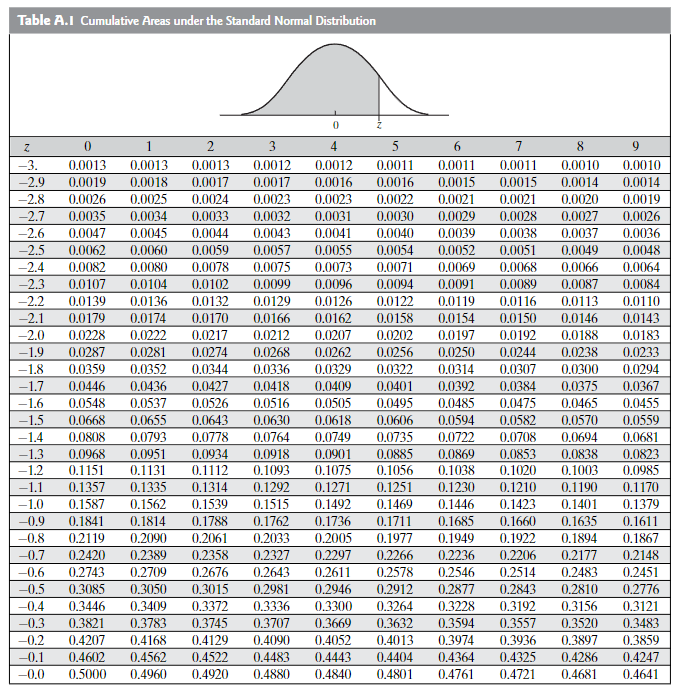
\includegraphics[width=\textwidth]{images/z-table_1.png}
    \caption{Cumulative Areas under the Standard Normal Distribution (Part 1)}
\end{figure}

\begin{figure}[ht]
    \centering
    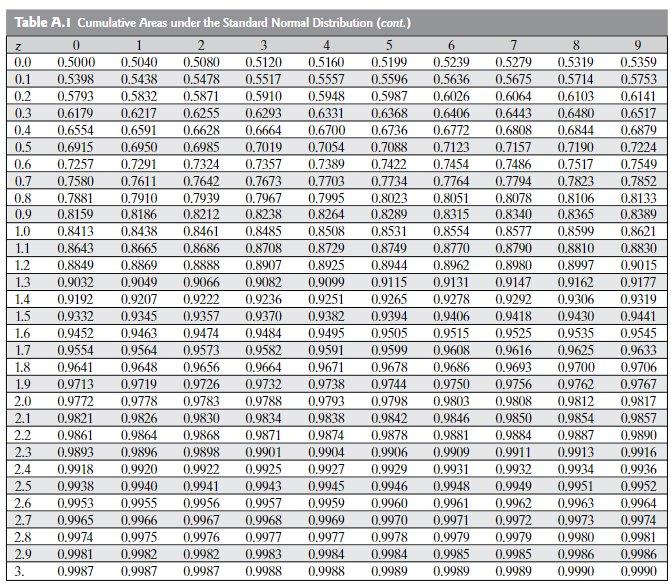
\includegraphics[width=\textwidth]{images/z-table_2.png}
    \caption{Cumulative Areas under the Standard Normal Distribution (Part 2)}
\end{figure}


\end{document}
